\chapter{Methodology}
\label{chap:methodology}

\section{Experiment Design}
The experiment proposal is tightly attached to the idea of using an eye-tracking 
system, not only because it is an innovation that gives us more precision within 
the measurements but it also uniqueness surrounding the state of the art as really 
few experiments have used this device. To be more exact we will be using the eye 
tracking model Tobii Pro Nano\cite{tobii_pro_nano}. The experiment is briefly described 
in this section, but it will be further explained in the chapter \ref{chap:experiment_execution}.

The user will be prompted with a text message showing the instructions. 
This text comes along with a previous tobii calibration that will be further 
explained in the section \ref{sub:eye-tracker_calibration} and \ref{sub:user_instructions} respectively. 
 
After the instructions and calibration are completed, the second phase, 
the actual experiment can start. There are two possible paths, 
negative display polarity path or positive display polarity path. Both 
affect the instruction texts as long as the screenshots shown to the user. The 
wiki text was shown always the first being followed by the product description. 
The user has as much time as they want.  However, it wasn’t possible to return to 
previous pages.

Once the user finished reading the third phase would start, a questionnaire regarding
 preference will be shown, it also contains a small set of questions about the texts
  to ensure the user has been reading carefully. 

In addition, the webpages chosen for the experiment are \url{wikipedia.org} and \url{amazon.es}. 
These two webpages will be further explained in the \ref{sub:reading_task} section. 
\section{Population of Study}
In order to have a good experiment, not only is it important to have a consistent and well-prepared 
process but also have a focus population of study. The decision was to check for university students 
as this was the easiest and most accessible population given the situation. Therefore, the objective 
age was young people between 18 to 30 years old.

It is also worth mentioning that the objective was to find the usual user on the internet. For that 
an average user isn’t a computer scientist as they can be specialized on web design or other similar 
fields. This point made us go to the faculty of Economics as it was a larger faculty and the students 
can be considered an “average” user.

The objective was to have 80 persons in total 20 women and 20 men divided evenly between the negative 
and positive display polarity. However, due to the lack of collaboration of the people and the tendency
 to decline collaboration in the experiment, this was later reduced to 34 in total.

To summarize, it can be concluded that the conditions and population of the study were:
\begin{table}[ht]
    \centering
    \caption{Distribution of participants by gender, polarity, and age.}
    \label{tab:participants}
    \small
    \setlength{\tabcolsep}{3pt} % Distancia fija para todos
    % Formula generada por Gemini para tener una tabla así de guapa, ni idea de que significa esa linea
    \begin{tabularx}{\textwidth}{|>{\raggedright\arraybackslash}p{2.2cm}|*6{>{\centering\arraybackslash}X|}>{\centering\arraybackslash}p{1.2cm}|}
        \hline
        %Fila 1 y 1.5
        \multirow{2}{*}{\makecell{\textbf{Number of} \\ \textbf{partic.}}} & \multicolumn{2}{c|}{\makecell{\textit{Neg.} 
        \\ \textit{Pol.}}} & \multicolumn{2}{c|}{\makecell{\textit{Pos.} \\ \textit{Pol.}}} & \multicolumn{2}{c|}
        {\textbf{\textit{TOTAL}}} & \multirow{2}{*}{\textbf{\textit{Age}}} \\ \cline{2-7}  % Lo ultimo es para la edad y su respectivo separador
         & Obj. & Act. & Obj. & Act. & Obj. & Act. & \\ \hline
        % fila 2
        \textit{Men} & 20 & 7 & 20 & 7 & 40 & 14 & \multirow{2}{*}{\makecell{[18,30]}} \\ \cline{1-7}
        % Fila 3
        \textit{Women} & 20 & 10 & 20 & 10 & 40 & 20 & \\ \hline
        %fila 4
        \textbf{\textit{Total}} & 40 & 17 & 40 & 17 & 80 & 34 & \\ \hline
    \end{tabularx}
\end{table}

\section{Tools}
In order to accomplish the success of the experiment there is a need of some tools. 
They will be further explained why they are important ant what purpose do they serve. 
There is one hardware tool requirement and 3 software tools that are used to collect 
data and process it.
\subsection{Tobii Pro Nano}
The tobii pro nano it’s an eye-tracker currently discontinued by the owners (Tobii)\cite{tobii_pro_nano} 
that is still to its day a great tool to collect user data. It’s worth mentioning that this 
tool is quite expensive and to use it the University of Oviedo has lent me one unit. Always
 with the surveillance of my tutors. The tobii pro nano is the lightest and most portable 
 unit offered, however it has some limitations that won’t be a problem in our case as the 
 limitations are for precise operations. 
 \begin{figure}
    \centering
    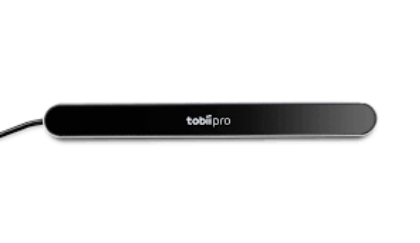
\includegraphics[width=0.5\textwidth]{figures/tobii_pro_nano.png}
    \caption{Tobii Pro Nano Device\cite{tobii_pro_nano}}
 \end{figure}
\subsubsection{Eye Tracker Technology Breakdown}
The eye tracker works in an amazing way, the process is a combination of high-quality cameras. 
Using what’s commonly called Pupil Center Corneal Reflection (PCCR). In the case of tobii pro 
nano it uses a patented variant of PCCR (US Patent US7,572,008).\cite{How_do_eyetrackers_work}

The PCCR is a mix between “illuminators” that is components that are almost infrared sensors 
that create such light on the eyes. Then different sets of cameras take pictures of the eye 
patterns and reflections. That is sent to algorithms that detect those patterns and reflections
 creating a detailed 3D model of the eye position and its gazes \cite{How_do_eyetrackers_work}.

\subsection{Tobii Pro Lab}
\begin{figure} [htb]
    \centering
    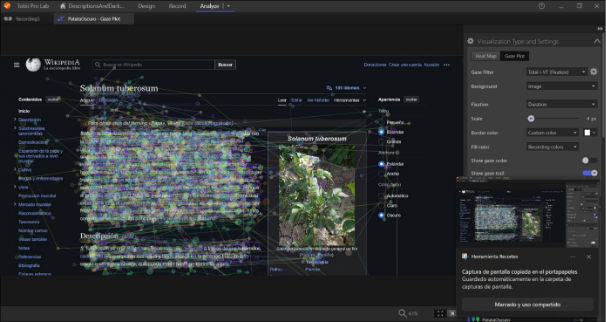
\includegraphics[width=0.5\textwidth]{figures/tobii_pro_lab.png}
    \caption{Tobii Pro Lab Software\cite{tobii_pro_lab}}
\end{figure}
The eye-tracking device connects to a software application called “Tobii Pro Lab”. This 
application aims to ease the use, collection and analysis of the gaze data. Curiously this is
 a negative display polarity program. It is needed to have a license in order to use it. 
 However, a 30 day trial is provided which has been enough toextract the data, change or create 
 the desired data, download it and process it. The data was gathered in the laptop of my proffesor
  as they have the paid license.Some of the most interesting tools are the visualization of heat maps, 
  recordings and the Areas of Interest, that will be further explained.

\subsection{Google Forms}
Google Forms is a free tool developed by Google that allows google users to create forms. This is a 
powerful tool as the answers can be stored in a Google Spreadsheet that can be exported as a .csv 
archive to be later processed. This tool is also pretty compatible with the tobii pro lab when creating 
the timelines that the user is going to be exposed due to the fact of the possibility of running.
\begin{figure}
    \centering
    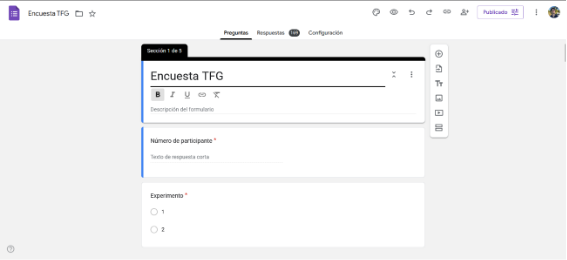
\includegraphics[width=0.5\textwidth]{figures/google_forms_example.png}
    \caption{Google Forms Example}
\end{figure}
\subsection{Python 3}
There’re few programming languages that almost everyone on earth has heard of, this is the case.
 Python is a powerful programming language not because of its speed or performance but because of
  the libraries that are available. This python environment makes room to one of the biggest spaces 
  for data processing. In my case, I’m not a specialized student on data processing, that’s why a 
  well-known and big space like this can be the perfect tool to approach a thesis. 
\subsubsection{Python external libraries}
As mentioned beforehand, the prowess of python resides in its libraries. The libraries used for this thesis are:
\begin{itemize}
    \item \textbf{Pandas}\cite{pandas}: Pandas is a library centered around the idea of easing
    data manipulation and analysis by providing a generic data structure called DataFrame. It is 
    almost an standard in the data ecosystem of python.
    \item \textbf{Matplotlib}\cite{matplotlib}: Matplotlib strength resides in its flexibility to 
    create any kind of graph. It is one of the most used libraries in Python.
    \item \textbf{NumPy}\cite{numpy}: NumPy name comes from “Numerical Python” and it is a library that provides 
    aid for the manipulation of arrays of data. It combines pretty well with Pandas as every column or row of a
    DataFrame can be transformed into a NumPy array easily.
    \item \textbf{SciPy}\cite{scipy}: SciPy is a library created for scientific and technical computing.
    Providing a large amount of functions for many different fields. In the case of this study, the biggest use
    resided in the statistics algorithms like Mann-Whitney U test and the t-test.
  \end{itemize}

\subsection{Dark Reader}
Given that the objective is to analyze the effects of display polarity on texts the decision was to
 choose a wiki page as it is a tool that until this day many users do. Moreover, an e-commerce is 
 another safe bet. In order to make it the most average the decision was to use “wikiedia.org” and
  “amazon.es”. However, the e-commerce website didn’t allow negative polarity, so we had to use a 
  firefox extension called Dark Reader which you can see in figure \ref{fig:dark_reader}

  \begin{figure}
    \centering
    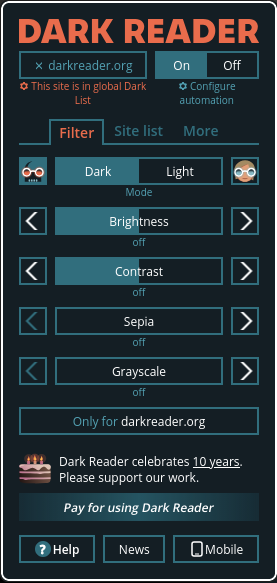
\includegraphics[width=0.5\textwidth]{figures/dark_reader.png}
    \caption{Dark Reader Extension\cite{dark_reader}}
    \label{fig:dark_reader}
  \end{figure}

\subsection{Python Web Interaction Behaviour (Pywib)}


Pywib\cite{clicks} is a python library desgined for the analysis of user behaviour within webpages. 
This library is still in development by a colleague of mine called Guillermo Dylan Carvajal and
despite of this tool is still in early stages, it is strong enough to be used in the analysis of this study.

TODO: Añadir más info sobre que funciones se han usado y para que sirven.